\documentclass{article} 
 %%%%%%%%%%%%%%%%%%%%%%%%%%%%%%%%%%%%%%%%%%%%%%%%%%%%%%%%%%%%
% PACKAGES
%%%%%%%%%%%%%%%%%%%%%%%%%%%%%%%%%%%%%%%%%%%%%%%%%%%%%%%%%%%%
\usepackage[utf8x]{inputenc}

% SYMBOLES
\usepackage{amsmath, amssymb, url} % amsthm, 

% ALGORITHMES
\usepackage[ruled,vlined,linesnumbered]{algorithm2e}



%%%%%%%%%%%%%%%%%%%%%%%%%%%%%%%%%%%%%%%%%%%%%%%%%%%%%%%%%%%%
% TIKZ
%%%%%%%%%%%%%%%%%%%%%%%%%%%%%%%%%%%%%%%%%%%%%%%%%%%%%%%%%%%%
\usepackage{pgf}
\usepackage{tikz}

\graphicspath{{./figures/}}

% Couleurs
\definecolor{turquoise}{rgb}{0 0.41 0.41}
\definecolor{rouge}{rgb}{0.79 0.0 0.1}
\definecolor{vert}{rgb}{0.15 0.4 0.1}
\definecolor{mauve}{rgb}{0.6 0.4 0.8}
\definecolor{violet}{rgb}{0.58 0. 0.41}
\definecolor{orange}{rgb}{0.8 0.4 0.2}
\definecolor{bleu}{rgb}{0.39, 0.58, 0.93}
\definecolor{gris}{rgb}{0.6,0.6,0.6}
\definecolor{grisfonce}{rgb}{0.4, 0.4, 0.4}
\definecolor{grispale}{rgb}{0.9, 0.9, 0.9}
% NOIR ET BLANC
\definecolor{vertfonce}{rgb}{0.0, 0, 0.0}
\definecolor{rougefonce}{rgb}{0, 0.0, 0.0}
\definecolor{rougeclair}{rgb}{0.6, 0.6, 0.6} %{red!50!white}
\definecolor{bleufonce}{rgb}{0.2, 0.2, 0.2} %blue!80!black
\definecolor{bleutresfonce}{rgb}{0.1, 0.1, 0.1} %blue!50!black
% \definecolor{vertfonce}{rgb}{0.0, 0.5, 0.0}
% \definecolor{rougefonce}{rgb}{1, 0.0, 0.0}
% \definecolor{rougeclair}{rgb}{1, 0.5, 0.5} %{red!50!white}
% \definecolor{bleufonce}{rgb}{0, 0, 0.8} %blue!80!black
% \definecolor{bleutresfonce}{rgb}{0, 0, 0.5} %blue!50!black


% Jeu de couleurs pales
% NOIR ET BLANC
\definecolor{cpale1}{rgb}{0.6, 0.6, 0.6}
\definecolor{cpale2}{rgb}{0.9, 0.9, 0.9}
% \definecolor{cpale1}{rgb}{1, 0.6, 0.6}
% \definecolor{cpale2}{rgb}{0.6, 1, 0.6}
\definecolor{cpale3}{rgb}{0.6, 0.6, 1}
\definecolor{cpale4}{rgb}{1, 0.6, 1}
\definecolor{cpale5}{rgb}{1, 1, 0.6}
\definecolor{cpale6}{rgb}{0.6, 1, 1}
\definecolor{cpale7}{rgb}{0.95, 0.65, 0.25}
\definecolor{cpale8}{rgb}{0.75, 0.45, 1}
\definecolor{cpale9}{rgb}{0.5, 1, 0.75}
\definecolor{cpale10}{rgb}{0.8, 0.7, 0.6}
\definecolor{cpale11}{rgb}{0.6, 0.7, 0.8}
\definecolor{cpale12}{rgb}{0.2, 0.5, 0.9}
\definecolor{cpale13}{rgb}{0.5, 0.9, 0.2}
\definecolor{cpale14}{rgb}{0.9, 0.2, 0.5}
\definecolor{cpale15}{rgb}{0.7, 0.7, 0.7}
\definecolor{cpale16}{rgb}{0.8, 0.8, 0.5}



%%%%%%%%%%%%%%%%%%%%%%%%%%%%%%%%%%%%%%%%%%%%%%%%%%%%%%%%%%%%
% CONSTANTES
%%%%%%%%%%%%%%%%%%%%%%%%%%%%%%%%%%%%%%%%%%%%%%%%%%%%%%%%%%%%

%-%-%-%-%-%-%-%-%-%-%-%-%-%-%-%-%-%-%-%-%-%-%-%-%-%-%-%-%-%
% CONSTANTES MATHEMATIQUES
%-%-%-%-%-%-%-%-%-%-%-%-%-%-%-%-%-%-%-%-%-%-%-%-%-%-%-%-%-%
% Booleens
\newcommand{\false}{{\tt false}}
\newcommand{\true}{{\tt true}}

% Ensembles
\newcommand{\AP}{\mathit{AP}}
\newcommand{\grandn}{{\mathbb N}}
\newcommand{\grandq}{{\mathbb Q}}
\newcommand{\grandqplus}{{\mathbb Q}_{\geq 0}}
\newcommand{\grandr}{{\mathbb R}}
\newcommand{\grandrplus}{\grandr_{\geq 0}}
\newcommand{\grandz}{{\mathbb Z}}
\newcommand{\setX}{\mathcal{K}_{\Clock}}
\newcommand{\setP}{\mathcal{K}_{\Param}}
\newcommand{\setXP}{\mathcal{K}_{\Clock \cup \Param}}

% Matrices
\newcommand{\matrixzero}{\mathbf{0}}
\newcommand{\matrixnopath}{\emptyset}

% Noms
\newcommand{\tiling}{\mathit{Tiling}}
\newcommand{\post}{\mathit{Post}}
\newcommand{\Pre}{\mathit{Pre}}
\newcommand{\TS}{\mathit{TS}}
\newcommand{\words}{\mathit{Words}}

% Operateurs
\DeclareMathOperator*{\argmax}{arg\,max}
\DeclareMathOperator*{\argmin}{arg\,min}
\newcommand{\eqdef}{ \overset{\mathit{def}}{=}}


% Symboles
\newcommand{\cro}[1]{\langle #1 \rangle}
\newcommand{\fleche}[1]{\stackrel{#1}{\rightarrow}}
\newcommand{\Fleche}[1]{\stackrel{#1}{\Rightarrow}}
\newcommand{\prefix}[2]{ |#1|_{#2} }
\newcommand{\steps}[0]{ {\rightarrow} }
\newcommand{\Steps}[0]{ {\Rightarrow} }
\newcommand{\timelaps}[1]{#1^\uparrow}
\newcommand{\trace}[1]{ \mathbin{<}#1 \mathbin{>}}
\newcommand{\wpi}[1]{\mathbin{<}#1\mathbin{>}}

% Temporal logics
\newcommand{\tlAlways}{\Box}
\newcommand{\tlEvt}{\Diamond}
\newcommand{\tlExists}{\exists}
\newcommand{\tlForall}{\forall}
\newcommand{\tlNext}{\bigcirc} % X
% \newcommand{\tlNext}{\circle}
\newcommand{\tlUntil}{\cup}

% Unites
\newcommand{\micros}{\mathit{\mu\,s}}
\newcommand{\millis}{\mathit{m\,s}}
\newcommand{\nanos}{ns}
\newcommand{\picos}{ps}


% Variables
\newcommand{\A}{\mathcal{A}}
\newcommand{\Avar}{\A_\mathit{var}}
\newcommand{\Clock}{X} % set of clocks
\newcommand{\clock}{x} % clock
\newcommand{\clockval}{w} % clock valuation
\newcommand{\enabled}{\mathit{enabled}}
\newcommand{\events}{E} % a possible set of events
\newcommand{\EventsSet}{\Sigma} % all possible events
\newcommand{\formule}{\varphi}
\newcommand{\Formule}{\Phi}
% \newcommand{\Kinit}{K_\mathit{init}} % initial constraint on the parameters
\newcommand{\LTS}{\mathcal{L}}
\newcommand{\Param}{P} % set of parameters (P / Y)
\newcommand{\param}{p} % parameter (p / y)
\newcommand{\py}{\pi} % parameter valuation
\newcommand{\Py}{\Pi} % set of consistent parameter valuations
\newcommand{\sinit}{s_\mathit{init}} % initial set of states
\newcommand{\Slast}{S_\mathit{last}}



\newcommand{\Ko}{K}
\newcommand{\pio}{\pi_0}
\newcommand{\piprime}{\pi}
\newcommand{\To}{T_0}
\newcommand{\Tprime}{T}


% \newcommand{\compyes}{\textcolor{green}{yes}}
\newcommand{\compyes}{$\textcolor{vertfonce}{\mathbf{\surd}}$}
% \newcommand{\compno}{\textcolor{red}{no}}
\newcommand{\compno}{$\textcolor{rougefonce}{\mathbf{\times}}$}


% Pour MDP
\newcommand{\we}{w}
\newcommand{\We}{W}
\newcommand{\va}{v}
\newcommand{\Va}{V}
\newcommand{\prob}{\mathit{Prob}}

%-%-%-%-%-%-%-%-%-%-%-%-%-%-%-%-%-%-%-%-%-%-%-%-%-%-%-%-%-%
% PARAMETRES
%-%-%-%-%-%-%-%-%-%-%-%-%-%-%-%-%-%-%-%-%-%-%-%-%-%-%-%-%-%
% PARAMETRES BRP
\newcommand{\brpMAX}{\mathit{MAX}}
\newcommand{\brpSYNC}{\mathit{SYNC}}
\newcommand{\brpTD}{\mathit{TD}}
\newcommand{\brpTR}{\mathit{TR}}
\newcommand{\brpTun}{\mathit{T1}}

% PARAMETRES CSMACD
\newcommand{\slot}{\mathit{slot}}

% PARAMETRES FLIP FLOP
\newcommand{\THold}{T_{\mathit{Hold}}}
\newcommand{\TSetup}{T_{\mathit{Setup}}}
\newcommand{\THI}{T_{\mathit{HI}}}
\newcommand{\TLO}{T_{\mathit{LO}}}
\newcommand{\TCKQ}{T_{ \mathit{CK} \rightarrow Q}}

% PARAMETRES RCP
\newcommand{\rcpFMax}{\mathit{f\_max}} % \mathit{rc\_fast\_max}
\newcommand{\rcpFMin}{\mathit{f\_min}} % \mathit{rc\_fast\_min}
\newcommand{\rcpSMax}{\mathit{s\_max}} % \mathit{rc\_slow\_max}
\newcommand{\rcpSMin}{\mathit{s\_min}} % \mathit{rc\_slow\_min}
\newcommand{\rcpD}{\mathit{delay}}

% PARAMETRES SIMOP
\newcommand{\COMct}{\mathit{COMct}}
\newcommand{\COMd}{\mathit{COMd}}
\newcommand{\NETd}{\mathit{NETd}}
\newcommand{\PLCct}{\mathit{PLCct}}
\newcommand{\PLCmtt}{\mathit{PLCmtt}}
\newcommand{\RIOd}{\mathit{RIOd}}
\newcommand{\SIGmrt}{\mathit{SIGmrt}}

% PARAMETRES SPSMALL
\newcommand{\tSetupA}{t_\mathit{setup}^A}
\newcommand{\tSetupD}{t_\mathit{setup}^D}
\newcommand{\tSetupWen}{t_\mathit{setup}^\mathit{WEN}}


% PARAMETRES WLAN
\newcommand{\pACK}{\mathit{ACK}}
\newcommand{\pACKTO}{\mathit{ACKTO}}
\newcommand{\pASLOTTIME}{\mathit{ASLOTTIME}}
\newcommand{\pBOFF}{\mathit{BOFF}}
\newcommand{\pDIFS}{\mathit{DIFS}}
\newcommand{\pMAXCOL}{\mathit{MAXCOL}}
\newcommand{\pSIFS}{\mathit{SIFS}}
\newcommand{\pTRANSTIMEMIN}{\mathit{TTMIN}}
\newcommand{\pTRANSTIMEMAX}{\mathit{TTMAX}}
\newcommand{\pVULN}{\mathit{VULN}}


%-%-%-%-%-%-%-%-%-%-%-%-%-%-%-%-%-%-%-%-%-%-%-%-%-%-%-%-%-%
% ALGORITHMES
%-%-%-%-%-%-%-%-%-%-%-%-%-%-%-%-%-%-%-%-%-%-%-%-%-%-%-%-%-%
% Algorithmes PTA
\newcommand{\IM}{\mathit{IM}}
\newcommand{\IMincl}{\IM_\subseteq}
\newcommand{\IMK}{\IM^K}
\newcommand{\IMunion}{\IM^\cup}
\newcommand{\IMinclK}{\IM^K_\subseteq}
\newcommand{\IMinclunion}{\IM^\cup_\subseteq}
\newcommand{\IMotf}{\IM_\mathit{otf}}
\newcommand{\BC}{\mathit{BC}}
\newcommand{\BCincl}{\BC_\subseteq}
\newcommand{\BCK}{\BC^K}
\newcommand{\BCunion}{\BC^\cup}
\newcommand{\BCinclK}{\BC^K_\subseteq}
\newcommand{\BCinclunion}{\BC^\cup_\subseteq}


%-%-%-%-%-%-%-%-%-%-%-%-%-%-%-%-%-%-%-%-%-%-%-%-%-%-%-%-%-%
% CONSTANTES DE CHAINES
%-%-%-%-%-%-%-%-%-%-%-%-%-%-%-%-%-%-%-%-%-%-%-%-%-%-%-%-%-%

% Langue
\newcommand{\absurde}{\emph{reductio ad absurdum}}

% Divers (projets et technique)

\newcommand{\lipsix}{LIP\,6}
\newcommand{\parissix}{Universit\'e Pierre et Marie Curie}
\newcommand{\simop}{SIMOP}
\newcommand{\spsmall}{SPSMALL}
\newcommand{\stm}{ST-Microelectronics}
\newcommand{\therac}{Therac-25}
\newcommand{\valmem}{VALMEM}

% Outils
\newcommand{\apron}{\textsc{Apron}}
\newcommand{\gdot}{\textsc{dot}}
\newcommand{\graphviz}{Graphviz}
\newcommand{\hytech}{{\sc HyTech}}
\newcommand{\imitator}{\textsc{Imitator}}
\newcommand{\imitatordeux}{\textsc{Imitator}\,II}
% \newcommand{\hymitator}{\textsc{Hymitator}}
\newcommand{\kronos}{\textsc{Kronos}}
\newcommand{\nusmv}{NuSMV}
\newcommand{\ocaml}{OCaml}
\newcommand{\phaver}{PHAVer}
\newcommand{\plot}{gnuplot}
\newcommand{\polka}{NewPolka}
\newcommand{\prism}{\textsc{Prism}}
\newcommand{\python}{Python}
\newcommand{\red}{RED}
\newcommand{\romeo}{Rom\'eo}
\newcommand{\smv}{SMV}
\newcommand{\spin}{Spin}
\newcommand{\tina}{TINA}
\newcommand{\trex}{\textsc{TReX}}
\newcommand{\uppaal}{\textsc{Uppaal}}
\newcommand{\vhdlta}{\textsc{Vhdl2Ta}}


% 
% \usepackage{pgf} 
% \usepackage{tikz} 
% \usetikzlibrary{arrows,automata} 
% \usepackage[latin1]{inputenc} 
% % \usepackage{verbatim} 
% % \usepackage{rtsched}


\title{Scheduling with IMITATOR: Some Case Studies}
\author{Romain Soulat}
\date{}
\begin{document}
\maketitle

\begin{abstract}
% 	We present here \imitator{} 2.5.
	The tool \imitator{}  implements the {\em Inverse Method} ($\IM$) for Timed Automata (TAs).
	Given a TA~$\A$ and a tuple $\pio$ of reference valuations for timings,
	$\IM$ synthesizes a constraint around  $\pio$ where $\A$ behaves in the same discrete manner.
	This provides us with a quantitative measure of robustness of the behavior of $\A$ around $\pio$.
	The new version \imitator{} 2.5 integrates the new features of stopwatches (in addition to standard clocks) and updates (in addition to standard clock resets), as well as powerful algorithmic improvements for state space reduction.
	These new features make the tool well-suited to analyze the robustness of solutions in several classes of preemptive scheduling problems.
\end{abstract}

%%%%%%%%%%%%%%%%%%%%%%%%%%%%%%%%%%%%%%%%%%%%%%%%%%%%%%%%%%%%
%%%%%%%%%%%%%%%%%%%%%%%%%%%%%%%%%%%%%%%%%%%%%%%%%%%%%%%%%%%%
\section{Motivation}
%%%%%%%%%%%%%%%%%%%%%%%%%%%%%%%%%%%%%%%%%%%%%%%%%%%%%%%%%%%%
%%%%%%%%%%%%%%%%%%%%%%%%%%%%%%%%%%%%%%%%%%%%%%%%%%%%%%%%%%%%

% The specification and verification of real-time systems, involving concurrency and timing delays, are notoriously difficult problems.
% The correctness of such real-time systems usually depends on the values of these timing delays.
% One can check the correctness for one particular value for each delay, but this does not guarantee the correctness for other values.
% Actually, checking the correctness for all possible delays, even in a bounded interval, would require an infinite number of calls to the model checker, because those delays can have real (or rational) values.
% It is therefore interesting to consider that these delays are \emph{parameters} (unknown constants), and synthesize a constraint on these parameters guaranteeing a correct behavior.
We show in this report how to exploit solutions of scheduling problems for generating zones of robustness around these solutions. We represent the scheduling problems under the
form of a Timed Automaton (TA). Each schedule (interleaving of tasks) corresponds to a branch in the reachability tree of the TA. A typical solution (schedule) corresponds
 to the shortest path of this tree.
Using the given solution of a scheduling problem, we explain how to synthesize a robustness region around this solution inside which the interleaving of the given solution
 still corresponds to the shortest path. In order to do this, we use a parametric version of the original TA and apply \imitator{}.




\imitator{} 2.5 (for \emph{Inverse Method for Inferring Time AbstracT behaviOR}) is a tool for parameter synthesis in the framework of real-time systems based on the inverse method~$\IM$ for Parametric Timed Automata (PTAs).  % ,~\cite{ad94}
Different from CEGAR-based methods% (see \cite{cgjlv00})
, this algorithm for parameter synthesis makes use of a ``good'' parameter valuation~$\pio$ instead of a set of ``bad'' states~\cite{acef09}.
\imitator{} takes as input a network of PTAs with stopwatches
and a reference valuation~$\pio$; it synthesizes a constraint~$\Ko$ on the parameters such that (1) $\pio \models \Ko$ and (2) for all parameter valuation~$\piprime$ satisfying $\Ko$, the trace set (i.e., the discrete behavior) of~$\A$ under~$\piprime$ is the same as for~$\A$ under~$\pio$.
%This preserves in particular linear time properties, 
This provides the system with a criterion of \emph{robustness} (see, e.g., \cite{m11})
%, by formally guaranteeing a uniform discrete behavior 
around~$\pio$.

% It , that synchronize on shared actions
% The input syntax, inspired by~\hytech{}, allows the use of clocks (or stopwatches), rational-valued discrete variables, and parameters (i.e. unknown constants) to be used altogether in linear terms, within guards, invariants and updates.

% By iterating the inverse method on all integer points within a bounded reference parameter domain, we get a set of constraints %(``tiles'')
% such that, for every point in each such constraint, the time-abstract behavior is the same: this gives a behavioral cartography of the system~\cite{af10}.



%-%-%-%-%-%-%-%-%-%-%-%-%-%-%-%-%-%-%-%-%-%-%-%-%-%-%-%-%-%-%
\begin{figure}[ht!]
	% STYLES
	\tikzstyle{etiquette} = [draw=none, color=black]
	
% \tikzstyle{boite}=[text width=8em, text centered, minimum height=2.5em, rounded corners, very thick]
% \tikzstyle{input}=[boite, draw=green!20!gris, top color=green!50, bottom color=green!10!white]
% \tikzstyle{output}=[boite, draw=red!20!gris, top color=red!50, bottom color=red!5!white]
% \tikzstyle{imitator} = [boite, draw=blue!20!gris, text width=10em, minimum height=6em]

	
	\tikzstyle{boite}=[rectangle, draw=black, rounded corners, thick, draw=blue!40!black, top color=blue!20, bottom color=blue!5!white]
% 	\tikzstyle{imitator} = [boite]
% 	\tikzstyle{apron} = [boite, draw=yellow!20!gris, top color=yellow!70, bottom color=yellow!10!white]
% 	\tikzstyle{polka} = [apron]
% 	\tikzstyle{ppl} = [apron]
	\tikzstyle{dot} = [boite, draw=purple!20!gris, top color=purple!60, bottom color=purple!10!white]

	\tikzstyle{fleche} = [->, draw=black, semithick]
{

\centering

\begin{tikzpicture}[scale=0.6,  =>stealth']

	% Boites
	\draw[boite] (-5, 5.5) rectangle (-2, 6.5);
	\node [etiquette] at (-3.5, 6) {PTA};
	
	\draw[boite] (-5, 3.8) rectangle (-2, 5);
	\node [etiquette] at (-3.5, 4.4) {\begin{tabular}{c}Reference\\valuation $\pio$\end{tabular}};
	
	\draw[boite] (0, 4) rectangle (6, 6.5);
	\node [etiquette] at (3, 5.25) {\large \imitator{}};
	
% 	\draw[boite] (1, 4) rectangle (5, 5);
% 	\node [etiquette] at (3, 4.5) {PPL};
	
	\draw[boite] (8, 4.5) rectangle (12, 6);
	\node [etiquette] at (10, 5.25) {Constraint $\Ko$};
	
% 	\draw[boite] (8, 4) rectangle (12, 5);
% 	\node [etiquette] at (10, 4.5) {Trace set};

	% Fleches
	\path[fleche] (-2, 6) --++ (2, 0);
	\path[fleche] (-2, 4.4) --++ (2, 0);
% 	\path[fleche] (3.5, 4) --++ (0, -.5);
% 	\path[fleche] (2.5, 3.5) --++ (0, .5);
	\path[fleche] (6, 5.25) --++ (2, 0);
% 	\path[fleche] (6, 4.5) --++ (2, 0);

\end{tikzpicture}

}

\caption{Functional view of \imitator{}}
\label{fig:structure}
\end{figure}
%-%-%-%-%-%-%-%-%-%-%-%-%-%-%-%-%-%-%-%-%-%-%-%-%-%-%-%-%-%-%
The plan of this paper is as follows. In section etc....



\section{Sketch of the Method illustrated on an example}
\label{sec:sketch}



Due to the aforementioned state space reduction and the use of stopwatches, \imitator{} 2.5 becomes an interesting tool for synthesizing robust conditions 
for scheduling problems.
Let us illustrate this on a preemptive jobshop example given in \cite{AM02}.
%In \cite{AM02}, the preemptive scheduling problem is encoded into TAs with stopwatches.
The jobshop scheduling problem is a generic resource allocation problem in which common resources (``machines'') are required at various time points (and for given duration) by different tasks.
For instance, one needs to use a machine $m_1$ for $d_1$ time units, machine $m_2$ for $d_2$ time units, and so on.
The goal is to find a way (``schedule'') to allocate the resources such that all tasks terminate as early as possible (``minimal makespan'').
% Given a fixed set $M$ of resources, a \emph{step} is a pair $(m,d)$ where $m \in M$ and $d \in \mathcal{N}$, indicating the required utilization of resource $m$ for time duration $d$.
% A \emph{job specification} is $J = (m_1,d_1),(m_2,d_2),\cdots, (m_k,d_k)$, stating that in order to accomplish job $J$, one needs to use a machine $m_1$ for $d_1$ time units, then use machine $m_2$ for $d_2$ time units, and so on.
%
Let us consider the jobshop problem $\{J_1, J_2\}$ for 2 jobs and 3 machines  with: $J_1 = (m_1,d_1), (m_2,d_2),(m_3,d_3)$ and $J_2 = (m_2,d'_2)$ with $d_1 = 3, d_2=2, d_3=4, d'_2 = 5$.
There are many possible schedules (two of them are depicted in Figure~\ref{fig:schedules_maler} in Appendix). 
%
% The problem is to find a schedule such that the value of the last completed job is minimal.
% This minimal value is called makespan.
% There are plenty techniques designed to solve this makespan problem.
In  \cite{AM02}, this problem is modeled as a product $\A$ of TAs with stopwatches, each TA modeling a job.
Each schedule corresponds to a branch in the reachability tree of~$\A$.
The makespan value corresponds to the
duration of the shortest branch, here~9.
% As a recapitulation, we have:
% \begin{itemize}
% 	\item Model $M$: A product of TAs
% 	\item Input $I$:  $\{(m_{i,j},d_{i,j})_{j\in J(i)}\}_{i \in \mathcal{I}}$
% 	\item Output: $\mu =$ minimal makespan
% \end{itemize}
% 
% For example, the makespan is found to be equal to 9.


Let us explain how to analyze the robustness of the
valuation $\pio:\{d_2=2,d'_2=5\}$ with respect to the makespan value 9.
% \subsection{Robustness Analysis}
We first consider a parametric version of ${\cal A}$ where
$d_2$ and $d'_2$ become parameters.
%In order to synthesize a constraint $K$ on parameters $d_2,d'_2$
%such that the minimum makespan value remains (at most) equal to 9,
In the same spirit as in \cite{cpr08},
we add an observer ${\cal O}$, which is a TA
synchronized with $\A$, that fires a transition labeled $\mathit{DEADLINE}$ as soon as a schedule spends more than 9 time units.
We then use \imitator{} (instead of a CEGAR-like method
as in \cite{cpr08}) with $\A \parallel {\cal O}$ as a model input
and $\pio$ as a valuation input.
This yields the constraint $\Ko$:  $7 > d'_2 \wedge 3 > d_2 \wedge d'_2 + d_2 \geq 7$.
(For a geometrical representation of~$\Ko$, see Figure~\ref{fig:geom} of Appendix 1.)
By the $\IM$ principle, the set of traces (i.e., discrete runs) of
$\A \parallel {\cal O}$ is always the same,
for any point $(d_2,d'_2)$ of~$\Ko$.
(This set of traces is depicted under the form of a tree in Figure~\ref{fig:output} in Appendix 1.)
Since the makespan for $\pio$ is~9,
we know that some branches of the tree do not contain
any $\mathit{DEADLINE}$ label (these branches end at node $s73$
in Figure~\ref{fig:output}).
This holds for each point $(d_2,d'_2)$ of~$\Ko$.
The makespan of the system is thus always at most~9 in~$\Ko$. (In particular, we can increase $d_2$ from 2 to 3, or increase $d'_2$ from 5~to~7
while keeping the makespan less than or equal to 9.)

%(in particular, when $d'_2 = 5$ and $d_2$ grows from 2 to 3, or $d_2 = 2$ and $d'_2$ grows from 5 to 7).

%This gives us a measure of robustness of the system around $\pio$.

% Such a robustness analysis, inspired from \cite{cpr08}, 
% has been conducted with \imitator{} 2.5
% on several classes of scheduling problems (see Table~\ref{table:results} in Appendix).

Another example of application of \imitator{} 2.5 to a scheduling problem, originating from \cite{bb04}, is given in Appendix 2 (using 
the cartography method of~\cite{af10}). 
All case studies and experiments %(performed on Ubuntu 11.10 equipped with an Intel Core\,2 2.93\,GiHz processor with 2\,GiB RAM)
are described in a research report~\cite{soulat12}. See also \url{http://www.lsv.ens-cachan.fr/Software/imitator/}.
%  (Source code, binaries, all case studies and logs are available in \url{http://www.lsv.ens-cachan.fr/Software/imitator/}).



%This gives us a quantitative measure of robustness of $\pio$,
%seen as a solution for the value 9 of makespan.
%.%for the input valuation $\pi_0 = \{d_2=2, d'_2 = 5\}$.
%By considering as reference parameter valuation~$\pio$ the duration for each task, and knowing the minimal makespan, one can use~$\IM$ in order to infer a constraint~$\Ko$ on the delays associated with each task.
%This gives a value of the robustness or implementability of the system, in the sense that, for any parameter valuation satisfying~$\Ko$, the system will be guaranteed to behave the same as for~$\pio$.
% We first transform the instantiated problem by parametrizing some of the duration values.
% In the example, we will consider that $d_2$ and $d'_2$ are parameters. We consider accordingly
%In order to ensure that~$\Ko$ preserves the schedulability under~$\pio$, one needs to represent the schedulability as a time-abstract behavior.
%  the parametric version $\mathcal{PA}$ of the original TA. Besides, we consider the makespan (viz, 9) as an additional input, and we construct a simple test automaton which is composed with $\mathcal{PA}$ in order to test wether or not the 
% last job is completed within the makespan.
% Finally, we give to IMITATOR as inputs:
% \begin{enumerate}
%  \item  the automaton resulting from the product of $\mathcal{PA}$ with the test automaton
%  \item  an input valuation $\pi_0 = \{d_2=2, d'_2 = 5\}$ for the parameters.
% \end{enumerate}
%We apply \imitator{} to a network of PTAs with stopwatches corresponding to the example of~\cite{AM02} (with only two parameters $d_2$ and $d'_2$).
% 
% \imitator{} outputs:
%  $ 7 > d'_2 \wedge 3 > d_2 \wedge d'_2 + d_2 \geq 7$.\footnote{There three couples of integer values that satisfy $K$: $(1,6)$, $(2,5)$, $(2,6)$...} This gives us a quantitative
%  measure of robustness for the input valuation $\pi_0 = \{d_2=2, d'_2 = 5\}$.
% 
% \begin{enumerate}
%  \item $(2,5) \in K$
%  \item the makespan of the system obtained by replacing $d_2, d'_2$ by $v_2, v'_2$ is less than or equal to 9, for all $(v_2,v'_2) \in K$.
% \end{enumerate}
% On this example K is equal to $ 7 > d'_2 \wedge 3 > d_2 \wedge d'_2 + d_2 \geq 7$.\footnote{There three couples of integer values that satisfy $K$: $(1,6)$, $(2,5)$, $(2,6)$.}
% \section{Presentation of the case studies}



% \subsection{Instantiated Problem}
In \cite{am02} Abdedda\"{i}m et Maler have shown how to encode the preemptive scheduling using Timed Automata with stopwatches (denoted here by TA). The Job-shop scheduling problem is a generic 
resource allocation problem in which common
resources (``machines'') are required at various time points (and for given duration) by different tasks. The goal is to find a way to allocate the resources such that all the tasks terminate
as soon as possible (or ``minimal makespan'' in the scheduling jargon). We consider a fixed set $M$ of resources. A \emph{step} is a pair $(m,d)$ where $m \in M$ and $d \in \mathcal{N}$, indicating 
the required utilization of resource $m$ for time duration $d$. A \emph{job specification} is a finite sequence
$$J = (m_1,d_1),(m_2,d_2),\cdots, (m_k,d_k)$$ of steps stating that in order to accomplish job $J$, one needs to use a machine $m_1$ for $d_1$ time, then use machine $m_2$ for $d_2$ time etc.
For details, see \cite{am02}.
For example, consider the job-shop problem with 2 jobs on 3 machines defined by $\{J_1, J_2\}$ with $J_1 = (m_1,d_1), (m_2,d_2),(m_3,d_3)$ and $J_2 = (m_2,d'_2)$ with $d_1 = 3, d_2=2, d_3=4, d'_2 = 5$.
There are many possible schedules; two of them are illustrated in Figure. \ref{fig:schedules_maler}.
\begin{figure}[!ht]
 \label{fig:schedules_maler}
 \caption{Schedules}
\end{figure}
The problem is to find a schedule such that the value of the last completed job is minimal. This minimal value is called makespan. There are plenty techniques designed to solve this makespan problem. In 
\cite{am02}, the authors show that the system can be modeled as a product of TAs, each TA corresponding to a job. The makespan problem then reduces to find the shortest path in the product.
As a recapitulation, we have:
\begin{itemize}
 \item Model $M$: A product of TAs
 \item Input $I$:  $\{(m_{i,j},d_{i,j})_{j\in J(i)}\}_{i \in \mathcal{I}}$
 \item Output: $\mu =$ minimal makespan
\end{itemize}

For the example, the makespan is found to be equal to 9.

% \subsection{Robustness Analysis}

We, now, explain how, using \imitator{} we are going to synthesize a zone of robustness around the 
We first transform the instantiated problem by parametrizing some of the duration values. In the example, we will consider that $d_2$ and $d'_2$ are parameters. We consider accordingly
 the parametric version $\mathcal{PA}$ of the original TA. Besides, we consider the makespan (viz, 9) as an additional input, and we construct a simple test automaton which is composed with $\mathcal{PA}$ in order to test wether or not the 
last job is completed within the makespan.
Finally, we give to IMITATOR as inputs:
\begin{enumerate}
 \item  the automaton resulting from the product of $\mathcal{PA}$ with the test automaton
 \item  an input valuation $\pi_0 = \{d_2=2, d'_2 = 5\}$ for the parameters.
\end{enumerate}
As an output, IMITATOR gives us a constraint $K$ on $d_2, d'_2$ such that: 
\begin{enumerate}
 \item $(2,5) \in K$
 \item the makespan of the system obtained by replacing $d_2, d'_2$ by $v_2, v'_2$ is less than or equal to 9, for all $(v_2,v'_2) \in K$.
\end{enumerate}
On this example K is equal to $ 7 > d'_2 \wedge 3 > d_2 \wedge d'_2 + d_2 \geq 7$.\footnote{There three couples of integer values that satisfy $K$: $(1,6)$, $(2,5)$, $(2,6)$.} This gives us a quantitative
 measure of robustness for the input valuation $\pi_0 = \{d_2=2, d'_2 = 5\}$.
% \section{Presentation of the case studies}

\section{Cyclic Tasks with a given scheduling policy}
\label{sec:fp-edf}
\subsection{Context}
In this framework of case studies, we want to prove the schedulability of cyclic tasks on a single machine, we consider the preemptive framework, where a currently running task
can be interrupted by another one when it becomes activated and has a higher priority. Each task $\tau_i$ is defined by an offset $O_i \in \mathcal{N}$ (the time before the first release), 
a period $T_i \in \mathcal{N}$ (the amount of time between two releases), a deadline $D_i \in \mathcal{N} $ (the maximum timed allowed to perform the task) and a Worst Case Execution Time $C_i \in \mathcal{N}$ (the maximum of work required to 
execute the task).

Added to these automata, we have an a priori scheduling policy either Fixed Priority (FP) or Earliest Deadline First (EDF). The first policy gives to each task $\tau_i$ 
a priority $\mathcal{P}_i$ and when
two tasks are activated at the same time, the computational time is given to the highest priority. The EDF policy gives the computational time to the task that has its deadline coming
the sooner.

In this context, given a scheduler, the system is said to be \emph{schedulable} if each task $\tau_i$ is completed before $D_i$ time units after the beginning of its period. 
Actually because of the periodicity of the problem, we only have to ensure that it is schedulable within $lcm_{i\in \mathcal{I}}(T_i)$.

\subsection{Instantiated Problem}
The problem is the following: given a list of tasks $\{\tau_i\}_{i \in \mathcal{I}}$ $$\tau_i = (O_i,T_i,D_i,C_i),$$ is the system schedulable?\\
\begin{itemize}
 \item Model $M$: A TA per task and a TA for the scheduler
 \item Input $I$: $\{O_i,T_i,D_i,C_i\}_{i \in I}$
 \item Output: Yes/No
\end{itemize}


\subsection{Robustness Analysis}
The problem is parametrized typically by letting deadlines $D_i$s instantiated and parametrizing some of the $C_i$s, $O_i$s and $T_i$s.
\begin{itemize}
 \item Model $M'$: a set of PTA deduced from $M$ by parametrizing the values of interest
 \item Input: $I$ and an identified set of parameters
 \item Output: a constraint $K$ such that for every $\pi \models K$, the $\pi$-instantiated model $M'[\pi]$ is schedulable.
\end{itemize}


% 
% 
% We leave certain values of interest that may be altered by an environment or an adversary as parameters, such as the $C_i$, $O_i$ and $T_i$, to quantify what kind of variations around the reference values does not lead to 
% unschedulability. 
% 
% If the system is schedulable under the reference valuation of the parameters, the constraint output by IMITATOR will guarantee that for every valuation within this constraint, the system is still schedulable.
% Input: $\{O_i,T_i,D_i,C_i\}_{i \in I}$\\
% Output: Yes/No\\
% Model: A TA per task and a TA for the scheduler.
\section{Premptive scheduling on one machine with Fixed Priority and variable execution times \cite{sgl97}}
\label{sec:sgl97}
\subsection{Context}
The problem addressed here is how to determine whether every job in $n$ independent job chains, denoted $J_1, J_2, \cdots, J_n$ can complete in time when the jobs are scheduled on a processor according to a 
priority-driven algorithm. Roughly speaking, we let $J_{i,j}$ denote the $j$th job of the chain $J_i$. Each job $J_{i_j}$ has a fixed priority $\Phi_{i,j}$ and is preemptable. The execution time of $J_{i,j}$ is
in the range $[e^{-}_{i,j},e^{+}_{i,j}]$ with $e^{-}_{i,j},e^{+}_{i,j}$ in $\mathcal{N}$. The release time $r_{i,j}$ of job $J_{i,j}$ is set to an integer value. $J_{i,1}$ is ready for execution at its release time $r_{i,1}$; for each $j > 1$, $J_{i,j}$ cannot
execute until its immediate predecessor $J_{i,j-1}$ completes. For details, see \cite{sgl97}. 
% 
% 
% In this framework of case studies taken from \cite{sgl97}, we want to find the makespan for independant chain of tasks that needs to be done on a single machine.
% Each chain is composed by one or several tasks that need to be done. Each task in a chain cannot
% start until a required amount of time ($r$) has elapsed and until the previous task in the chain has not been completed (except for the first job of every chain). Each task has a Best Case Execution Time (BCET) denoted
%  by $e^{-}$ and a Worst Case Execution Time (WCET) denoted by $e^{+}$. Moreover, since there is only one machine, each task is given a priority $\Phi$ and the machine time is given to the task with the highest priority.
% This way, each chain is a list of tasks and can be given by $(r_{i,j},e^{-}_{i,j},e^{+}_{i,j},\Phi_{i,j})_{i\in I}$
\subsection{Instantiated Problem}
We are given a list of chain of tasks $\{J_i\}_{i \in \mathcal{I}}$ where $J_i = {J_{i,j}}_{j \in \mathcal{J}(i)}$ and $$J_{i,j} = (r_{i,j},e^{-}_{i,j},e^{+}_{i,j},\Phi_{i,j}).$$
The problem is: what is the minimum time needed to do all the chain of tasks?
\begin{itemize}
 \item Model: A product of TAs, with a TA per task and a TA for the FP scheduler
 \item Input: $I = (r_{i,j},e^{-}_{i,j},e^{+}_{i,j},\Phi_{i,j})_{i\in \mathcal{I}}$
 \item Output: $\Delta =$ Worst case completion time of the last task (of the last chain).
\end{itemize}

\subsection{Robustness Analysis}
The problem is parametrized typically by letting the priorities $\Phi_{i,j}$ and the $[e^{-}_{i,j},e^{+}_{i,j}]$ instantiated as well as the computed value $\Delta$, and by parametrizing some of the $r_i$s.

\begin{itemize}
 \item Model $M'$: a PTA deduced from $M$ by parametrizing the values of interest and composed with a TA that tests wether or not the last task is completed within $\Delta$ (using an error state)
 \item Input: $I$ together with $\Delta$ and an identified set of parameters 
 \item Output: a constraint $K$ such that for every $\pi \models K$, the last task of the $\pi$-instantiated model $M'[\pi]$ is completed within $\Delta$.

\end{itemize}



% 
% For IMITATOR, we take the same list of chain that was used in the original problem and the resulting makespan. We add a very simple automata that checks when every chain has been completed if it has been done in 
% less than the makespan and in this case the automaton goes to a success state, or in more time that required and in this case it goes to an error state.
% We leave certain values of interests that may be altered by an environment or an adversary as parameters, such as the $^{-}_{i,j}, \ e^{+}_{i,j}$ and $r_i$, to quantify what kind of variations around the reference values does not lead to being unschedulable within
% the makespan found for the original problem.
% 
% For any valuation within the constraint output by IMITATOR, there exists a scheduler such that the new makespan is less or equal to the original makespan.

\section{Cyclic Tasks with an FP scheduling policy and an error state \cite{cpr08,lpprc10}}
\label{sec:cpr08}
\subsection{Context}
if S is a periodic
task system, the activation automaton simply consists of a
network of n independent timed automata, each representing
the activation of periodic task $\tau_i$, as shown in Fig. \ref{fig:cyclic_task}; each task $\tau_i$ has a period $T_i$, a fixed duration of time between
two activation events, and it may have an offset $O_i$ for its first activation time. Its activation automaton contains
a clock, which is reset every time the period is reached
and $Release_i$ is fired. (This is depicted on Figure \ref{fig:cpr08-aut}.)

\begin{figure}[!ht]
 \centering
 \includegraphics[scale = 0.4]{./Figures/cppr08_automata.jpg}
 \caption{Automata for a cyclic task and a FP scheduler from \cite{cpr08}}
 \label{fig:cpr08-aut}
\end{figure}

When a job is activated, it executes
for at most a time $C_i$, and has to terminate within the
relative deadline $D_i$. The activation of jobs can be modeled by a parametric
timed automaton, where activation events are associated with transition labels, see Fig. \ref{fig:cyclic_task}.

A Fixed Priority scheduler automaton is added to these tasks. When the time
elapsed from the last activation of a task equals to its deadline
time and the total demanded time exceeds the length of
the interval, the task misses the deadline and the automaton reaches an error state. For details see n \cite{cpr08}.


\begin{figure}[!ht]
\centering
\label{fig:cyclic_task}
% \begin{tikzpicture}[->,>=stealth',shorten >=1pt,auto,node distance=6cm, 
%                     semithick] 
%     \tikzstyle{every state}=[fill=white,draw=black,text=black, text width = 1.33cm]
%    \tikzstyle{every edge}=[draw = black, text width = 4cm] 
%    \node[state] (I)                    {Init\\$t <= O$};
%    \node[state] (A)        [right of= I]            {idle\\$t <= T$};
%   \node[state]         (B) [right of=A]        {waiting/running\\$t <= T$}; 
%    
%    \path (A) edge [bend left=3]    node {$t = T$\ \\Require \ \\$t:= 0$} (B)
%          (B) edge [bend left=3]    node {Done } (A)
% 	 (I) edge [bend left=60]	 node {$t = O$\ \\Require \ \\$t:= 0$} (B);
% \end{tikzpicture}
 \caption{Automaton for a periodic task with an offset}
\end{figure}
We say that the system is \emph{schedulable} if each task $\tau_i$ is completed before its relative deadline $D_i$. Actually, because of the periodicity
of the system, we only have to be sure that it is schedulable within $lcm_{i\in I}(T_i)$.
% In this framework of case studies as presented in \cite{cpr08,lpprc10}, we want to prove the schedulability of cyclic tasks on a single machine. Each task is defined by an offset (the time before the first release), 
% a period (the amount of time between two releases), a deadline (the maximum timed allowed to perform the task) and a Worst Case Execution Time (the maximum of work required to 
% execute the task). These parameters are respectively denoted by $O$, $T$, $D$ and $C$. The main difference between this framework and the one in section I is that multiple occurence of the same task can 
% be active at the same time.
% 
% A Fixed Priority scheduler automata is added to these tasks. It has an error state, where it can go if the deadline is met and the required amount of work had not been performed.
% 
% The problem is said to be schedulable if there is a way to schedule tasks such that every task is accomplished during its own period and before its deadline.

\subsection{Instantiated Problem}
We are given a list of tasks $\{\tau_i\}_{i \in \mathcal{I}}$ with $$\tau_i=(O_i,T_i,D_i,C_i).$$ 
The problem is: is the system schedulable? 
\begin{itemize}
 \item Model $M$: A TA per task and a TA for the scheduler
 \item Input $I$: $\{O_i,T_i,D_i,C_i\}_{i \in I}$
 \item Output: Yes or No
\end{itemize}



\subsection{Robustness Analysis}
% We leave certain values of interests that may be altered by an environment or an adversary as parameters, such as the $C_i$, $O_i$ and $T_i$, to quantify what kind of variations around the reference values does not lead to 
% unschedulability. 
% If the system is schedulable under the reference valuation of the parameters, the constraint output by IMITATOR will guarantee that for every valuation within this constraint, the system is still schedulable.


The problem is parametrized typically by letting the deadlines $D_i$s instantiated and by parametrizing some of the $C_i$s, $O_i$s and $T_i$s.
\begin{itemize}
 \item Model $M'$: a PTA deduced from $M$ by parametrizing the values of interest 
 \item Input: $I$ and an identified set of parameters
 \item Output: a constraint $K$ such that for every $\pi \models K$, the $\pi$-instantiated model $M'[\pi]$ is schedulable.
\end{itemize}


\section{Premptive Job-Shop Scheduling with multiple machines \cite{am02}}
\label{sec:am02}
\subsection{Context}
The Job-shop scheduling problem is a generic resource allocation problem in which common
resources (``machines'') are required at various time points (and for given duration) by different tasks. The goal is to find a way to allocate the resources such that all the tasks terminate
as soon as possible (or ``minimal makespan'' in the scheduling jargon). We consider a fixed set $M$ of resources. A \emph{step} is a pair $(m,d)$ where $m \in M$ and $d \in \mathcal{N}$, indicating 
the required utilization of resource $m$ for time duration $d$. A \emph{job specification} is a finite sequence
$$J = (m_1,d_1),(m_2,d_2),\cdots, (m_k,d_k)$$ of steps stating that in order to accomplish job $J$, one needs to use a machine $m_1$ for $d_1$ time, then use machine $m_2$ for $d_2$ time etc. For details, see \cite{am02}.
% 
% In this framework of case studies presented in \cite{am02}, we want to find the makespan for independant chain of tasks that needs to be done on a several machines.
% Each chain is composed by one or several tasks that need to be done. Each task of the chain has a WCET (denoted by $C$). When two tasks try to work on the same machine, one has to preempt the other one. There is 
% no a priori scheduling policy so everything is possible.
% This way, each chain is a list of tasks and can be given by a list of couples $(m_i,C_i)$ where $m$ is the machine on which the task has to performed and $C$ the required amount of time to be spent on this machine
% in order to move to the next task.

\subsection{Instantiated Problem}
We are given a list of job specifications $\{J_i\}_{i \in \mathcal{I}}$ where $$J_i =\{(m_{i,j},d_{i,j})\}_{j \in J(i)}.$$ 
The problem is: What is the minimal makespan to complete all the chain of tasks?
\begin{itemize}
 \item Model $M$: A product of TAs, with a TA per job
 \item Input $I$:  $\{(m_{i,j},d_{i,j})_{i\in I(j)}\}_{j \in J}$
 \item Output: $\mu =$ minimal makespan
\end{itemize}


\subsection{Robustness Analysis}
The problem is parametrized typically by parametrizing some of the $d_i$s.


\begin{itemize}
 \item Model $M'$: a PTA deduced from $M$ by parametrizing the values of interest and composed with a TA that tests wether or not the last task is completed within $\mu$ (using an ok and an error state)\\
 \item Input: $I$ together with an identified set of parameters and the value of the computed makespan $\mu$ \\
 \item Output: a constraint $K$ such that for every $\pi \models K$, there is a schedule which allows to complete the last task of the $\pi$-instantiated model $M'[\pi]$ within $\mu$.
\end{itemize}

\section{Schedulability Analysis with Behavioral Cartography}
\label{sec:bb04}
When one is only interested in finding all the parameters valuation such that the system is schedulable, without considering a particular schedule, it is interesting to consider the Behavioral Cartography Method
included in IMITATOR. 
 By iterating $IM$ over all the integers points %(or each step given by a rational value, e.g., $1/3$)
inside a finite but dense rectangle $V_0$ in the parametric space, one is able to decompose (most of) the parametric space included into $V_0$ into behavioral tiles\footnote{Actually, one can take a finer discretization step than integers to ensure a better coverability of~$V_0$}~\cite{af10}.

For a given tile, we ensure that for every valuation of the parameters in this tile, the behavior of $\mathcal{A}$ is the same;
therefore, we only have to test the schedulability of a single point for each tile to ensure the schedulability on the whole tile.

Let us apply this method on a ``Rate monotonic'' example of \cite[Section~III]{bb04}.
There are three periodic tasks $\tau_1, \tau_2$ and $\tau_3$ with periods of $T_1 = 3, \ T_2 = 8$ and $T_3 = 20$ and deadlines of $D_1 = 3, \ D_2 = 8$ and $D_3 = 20$.
We are interested in finding the set of computation times of each task such that the system is schedulable.
(The interested reader can find the full details in \cite{bb04}.)

We set $V_0$ as $C_1 \in [0,3]$, $C_2 \in [0,8]$ and $C_3 \in [0,20]$, where $C_i$ is the computational time of $\tau_i$. The system is unschedulable if there exists a task $\tau_i$ such that $C_i > T_i$. 
% We recall the algorithm for $\BC$, we first pick an integer point $\pi_k$ that does not belong to any tile already computed and we synthesize $\IM(\A,\pi_k)$ which will be a new tile. We iterate this process 
% until no integer point remains uncover (since $V_0$ only contains a finite number of integer points, we know that GC will terminate in a finite number of iterations).
Algorithm~$BC$ outputs the set of tiles and we check for one point of each tile whether the system is schedulable or not.
The result for this example is given in Figures \ref{fig:carto1}, \ref{fig:carto2}, \ref{fig:carto3} for this $V_0$ with a discretization step of $0.2$.

\begin{figure}[!ht]
	\centering
 	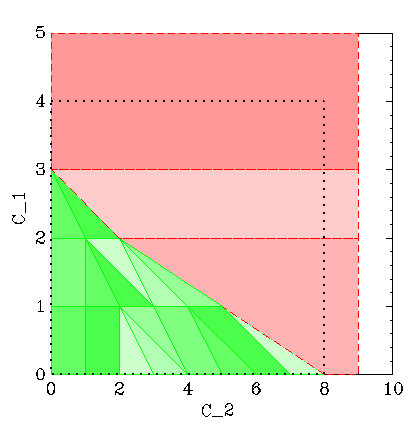
\includegraphics[scale = 0.5]{./Figures/C1-C2.png}
	\caption{Cartography output by IMITATOR 2.5 (in green the system is schedulable; in red, unschedulable)}
	\label{fig:carto1}
\end{figure}

\begin{figure}[!ht]
	\centering
 	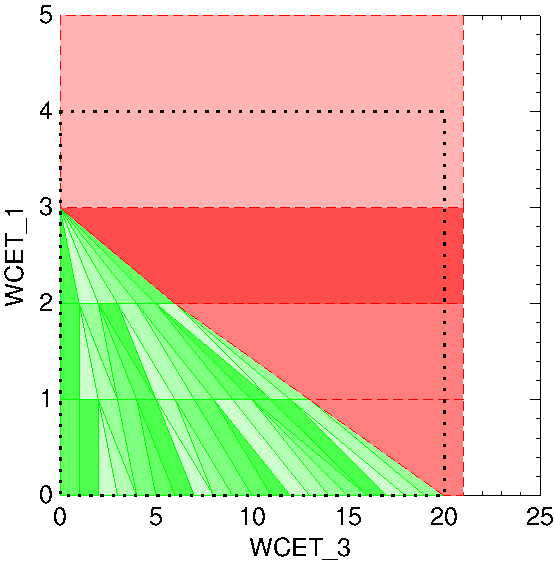
\includegraphics[scale = 0.4]{./Figures/C3-C1.png}
	\caption{Cartography output by IMITATOR 2.5 (in green the system is schedulable; in red, unschedulable)}
	\label{fig:carto2}
\end{figure}

\begin{figure}[!ht]
	\centering
 	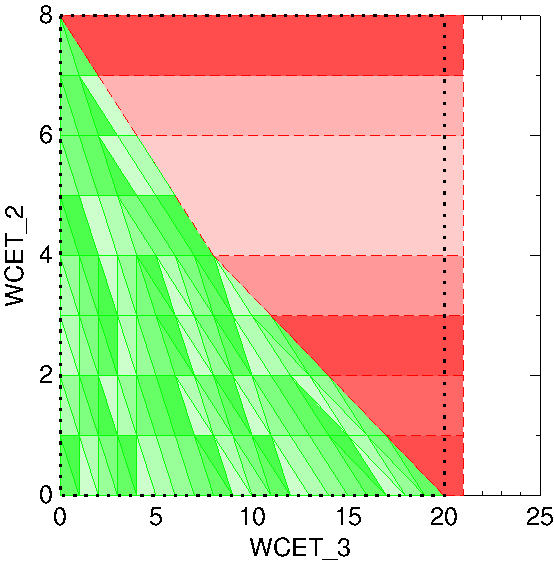
\includegraphics[scale = 0.4]{./Figures/C3-C2.png}
	\caption{Cartography output by IMITATOR 2.5 (in green the system is schedulable; in red, unschedulable)}
	\label{fig:carto3}
\end{figure}

\section{Results}
All case studies and experiments have been performed on Ubuntu 11.10 equipped with an Intel Core\,2 2.93\,GiHz processor with 2\,GiB RAM).
 See also \url{http://www.lsv.ens-cachan.fr/Software/imitator/}.
\begin{figure}[!ht]
\begin{tabular}{|c|c|c|c|c|c|c|c|c|}
\hline
 Case study 		& $|\mathcal{A}|$& $|X|$ & $|P|$ & $|s|$ 	& $|t|$ 	& $n$ 	& $|K|$ & t (s) 	      	\\
\hline
\multicolumn{9}{||c||}{Examples from section \ref{sec:fp-edf}}\\
\hline
FP 0	& 5 & 7 	& 10 	& 63 	& 62 	& 32 & 12 & 1.10  	\\
\hline
FP 1		& 5 & 7 	& 10 	& 205 	& 225	& 40	& 11 & 15.6  \\
\hline
FP 2		& 5 & 7 	& 10 	& 208  	& 228	& 42	& 12 & 10.7  \\
\hline
FP 3		& 5 & 7 	& 10 	& 49	& 51		& 15	& 12 & 1.03  \\
\hline
EDF 0 	& 5 & 10 	& 13 	& 63 	& 62 	& 32 & 13 & 2.42  	\\
\hline
EDF 1		& 5 & 10 	& 13 	& 76 	& 91 & 31	& 20 & 66.1  \\
\hline
EDF 2		& 5 & 10 	& 13 	& 254  	& 326	& 47	& 12 & 9.9  \\
\hline
EDF 3		& 5 & 10&  13   & 31 	& 33		& 9	& 13 & 1.09  \\
\hline
\multicolumn{9}{||c||}{Examples from section \ref{sec:sgl97}}\\
\hline
from \cite{sgl97}		 &8& 	15& 	18& 	215& 	264& 	15& 	17& 	85.3\\
\hline
\multicolumn{9}{||c||}{Examples from section \ref{sec:cpr08}}\\
\hline
from \cite{cpr08} &4 &	6 &	8 &	676& 	886& 	15& 	15& 	288.3\\
\hline
from \cite{lpprc10} &3 &	4 &	9 &	60& 	103& 	10& 	7& 	2.1\\
\hline
\multicolumn{9}{||c||}{Examples from section \ref{sec:am02}}\\
\hline
from \cite{am02} 	&3&	3& 	4& 	53& 	70& 	10& 	5& 	0.45\\
\hline 
LA02 2$\times$5	&3&	3&	11&	371&	528&	21&	10&	63.4\\
\hline
LA02 3$\times$5&	4&	3&	16&	4903&	9043&	30&	5	&160.6\\
\hline
\multicolumn{9}{||c||}{Examples from section \ref{sec:bb04}}\\
\hline
from \cite{bb04}	&5&	7&	10&	\_&	\_&	\_&	\_&	66\\
\hline

\end{tabular}
\caption{Results for the schedulability problem}
\end{figure}
The examples have been executed with the following commands:
\begin{itemize}
 \item For [AM02], [SGL97], [CPR08], [HPPR10], all examples from section 2:\\ IMITATOR case\_study.imi case\_study.pi0 -merge 
 \item For [LA02] 2$\times$5, [LA02] 3$\times$5:\\ IMITATOR case\_study.imi case\_study.pi0 -merge -inclusion 
 \item For the cartography of [BB04]:\\ IMITATOR case\_study.imi case\_study.v0 -mode cover -merge -step 0.2 
\end{itemize}

The examples LA02 2$\times$5 and 3$\times$5 are extracted from the LA02 example of \cite{am02}, we only consider the 2 (resp. 3) first jobs on 5 machines.
Faire reference a la page web
%%%%%%%%%%%%%%%%%%%%%%%%%%%%%%%%%%%%%%%%%%%%%%%%%%%%%%%%%%%%
%%%%%%%%%%%%%%%%%%%%%%%%%%%%%%%%%%%%%%%%%%%%%%%%%%%%%%%%%%%%
\section{Final Remarks}
%%%%%%%%%%%%%%%%%%%%%%%%%%%%%%%%%%%%%%%%%%%%%%%%%%%%%%%%%%%%
%%%%%%%%%%%%%%%%%%%%%%%%%%%%%%%%%%%%%%%%%%%%%%%%%%%%%%%%%%%%

%One of the first powerful model checkers for analyzing PTAs is \hytech{}~\cite{hhw97}.
%Unfortunately, it can hardly verify even medium sized examples due to exact arithmetics with limited precision and static composition of automata.
%%, quickly leading to memory overflows.
%%%Since, \trex{}~\cite{abs01} has been able to perform parameter synthesis%(see, e.g.,~\cite{cs01})
%, and 

The use of models such as PTAs and parametric Time Petri Nets (TPNs)
for solving scheduling problems has received attention in the past few years.
For example, \romeo{}~\cite{lrst09} performs 
%parametric model checking for TPNs
model checking for parametric TPNs with stopwatches, and synthesizes parameter valuations satisfying TCTL formul\ae{}.
An extension of \uppaal{} allows parametric model checking \cite{BLR05formats}, although the model itself remains non-parametric.
%See, e.g., Section\,7 of~\cite{cpr08} for a survey.
%
% \commentaire{
% ex italiens : assure schedulability (etat erreur jamais atteint, donc schedulable vis a vis d'une deadline) ; forme of robustness autour d'un point de depart connu comme schedulable
% }
%
The approach most related to \imitator{} 2.5 is~\mbox{\cite{cpr08,LPPRC10}}, where the authors infer parametric constraints guaranteeing the feasibility of a schedule, using PTAs with stopwatches.
The main difference between~\cite{cpr08,LPPRC10} and \imitator{} relies in our choice of the inverse method, rather than a CEGAR-based method.
First results obtained on the same case studies
are incomparable (although similar in form), which seems to indicate
that the two methods are complementary.
%%%Also, although \imitator{} 2.5 is well-suited to schedulability analysis, as emphasized here,
%%%the tool applies to many other classes of concurrent real-time systems, such as communication protocols and hardware components (see, e.g.,~\cite{acef09}).
%%%
The problem of finding the schedulability region was attacked in analytic terms
in \cite{bb04};
the size of our examples is rather modest compared to those treated using such analytic methods.
However, in many schedulability problems,
no analytic solution exists (see, e.g.,~\cite{SGL97}), 
and exhaustive simulation is exponential
in the number of jobs. In such cases, symbolic methods as ours and those
of \cite{cpr08,LPPRC10}  are useful to treat
critical real-life examples of small size.
We are thus involved in a project~\cite{fl11} with an industrial partner 
with first interesting results.

% A graphical user interface for the input model is currently under construction, based on a generic platform. \commentaire{utile ?!}

%\subsubsection*{Future Work}
%In~\cite{FK11}, $\IM$ has been extended to {\em hybrid} automata, and a prototype 
%based on \imitator{} 
%has been implemented.
%Bridging the gap between that %experimental 
%prototype with high expressiveness but moderate performances, and the optimized \imitator{} 2.5 dedicated to PTAs with stopwatches is the subject of ongoing work.





\bibliographystyle{plain}
\bibliography{biblio}
\newpage
\begin{appendix}
 \section{Parameter values for the FPs and EDFs examples}

\subsection{FP 0 and EDF 0}
Three cyclic tasks of the form $\tau_i = (O_i,T_i,D_i,C_i)$ with:
\begin{itemize}
 \item $\tau_1 = (0,10,10,4)$
 \item $\tau_2 = (94,100,100,20)$
 \item $\tau_3 = (0,1000,1000,120)$
\end{itemize}
and the priorities for FP 0 are $\mathcal{P}_1=3$, $\mathcal{P}_2=2$ and $\mathcal{P}_3=1$.

\subsection{FP 1 and EDF 1}
Three cyclic tasks of the form $\tau_i = (O_i,T_i,D_i,C_i)$ with:
\begin{itemize}
 \item $\tau_1 = (0,100,100,20)$
 \item $\tau_2 = (0,150,150,40)$
 \item $\tau_3 = (0,350,350,100)$
\end{itemize}
and the priorities for the FP 1 are $\mathcal{P}_1=3$, $\mathcal{P}_2=2$ and $\mathcal{P}_3=1$.

\subsection{FP 2 and EDF 2}
Three cyclic tasks of the form $\tau_i = (O_i,T_i,D_i,C_i)$ with:
\begin{itemize}
 \item $\tau_1 = (0,3,3,1)$
 \item $\tau_2 = (0,5,5,1)$
 \item $\tau_3 = (0,10,10,1)$
\end{itemize}
and the priorities for the FP 2 are $\mathcal{P}_1=3$, $\mathcal{P}_2=2$ and $\mathcal{P}_3=1$.

\subsection{FP 3 and EDF 3}
Three cyclic tasks of the form $\tau_i = (O_i,T_i,D_i,C_i)$ with:
\begin{itemize}
 \item $\tau_1 = (0,100,100,20)$
 \item $\tau_2 = (0,150,150,40)$
 \item $\tau_3 = (0,160,160,20)$
\end{itemize}
and the priorities for the FP 3 are $\mathcal{P}_1=3$, $\mathcal{P}_2=2$ and $\mathcal{P}_3=1$.

\end{appendix}

\end{document}
